\documentclass{article}
\usepackage{geometry}
\usepackage{graphicx}

\geometry{margin=1in}
\title{Lab 1 Report}
\author{Ty Davis, Chandler Griffith}

\begin{document}
\maketitle
We are building a simple rectifier circuit with a constant supply
voltage of 10 V and a 1 k$\Omega$ resistor. The point of this lab
is to analyze the operating voltage and current of a certain diode.
The diode we're using in this lab is the 1N4001 diode, and we're using
one manufactured by Texas Instruments.

\section{Calculation}
There are three models that we can use to analyze the diode in a 
circuit, they are the \emph{ideal}, \emph{constant drop}, and the
\emph{exponential} models.
\subsection{Ideal Model}
In the ideal model we assume that there is no voltage drop over
the diode, and that for any positive voltage across the diode, the
current is infinite.
We can use Ohm's Law to show the ideal model. This is $V=iR$.

This yields the following calculation. 
$$\frac{10 \textrm{ V}}{1 \textrm{k}\Omega} = 10 \textrm{ mA}$$
\subsection{Constant Drop Model}
For the constant drop model we assume that the voltage drop over the diode
is 0.7 V, which is close to the actual operating point. When the diode 
faces any voltage drop greater than 0.7 V, the current is assumed 
to be infinite.
We can use Ohm's Law while subtracting that constant voltage so 
that we get the following calculation.
$$\frac{10 \textrm{ V} - 0.7 \textrm{ V}}{1 \textrm{k}\Omega} = 9.3 \textrm{ mA}$$

\subsection{Exponential Model}
In the exponential model we use the equation $I_D=I_S e^{\frac{V_D}{V_{th}}}$ to find
the current through the diode. $V_{th}$ is known to be about 25.9 mA 
at about 300K, and we calculated $I_S$ from values measured from the 
physical circuit.

\section{Computer Calculation}
Using python and the measured values we graphed two equations. The 
two equations are $I_D = \frac{V_{DD} - V_D}{R}$ and $I_D = I_S e^{\frac{V_D}{V_{th}}}$. 
Those two equations are considered because we derive from Kirkhoff's 
Current Law as we describe the relationship between the current through
the resistor and the diode. The intersection of these two graphs shows the 
operating voltage and current of the diode.

In Figure 1 you can see the operating voltage of the diode is
calculated at V$=0.698$ V and I$=9.317$ mA. These figures align 
well with the measured values as you will see later in the lab.

\begin{figure}
  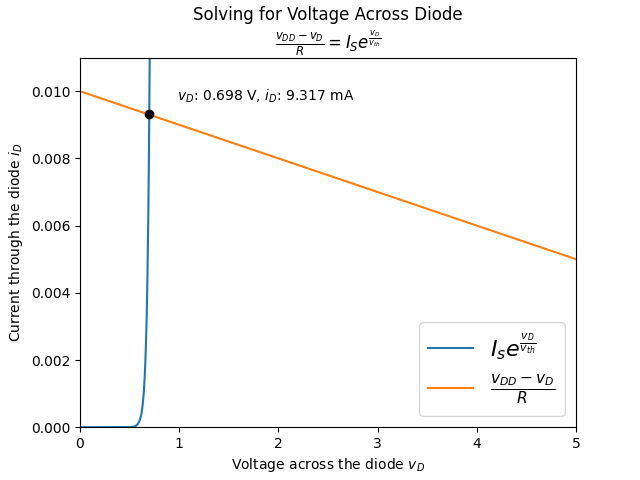
\includegraphics[width=0.7\linewidth]{out.png}
  \caption{Intersection of current graphs for Diode and Resistor}
  \label{fig:graph1}
\end{figure} 

\section{Simulation}
In Figure 2 we see the circuit that was modeled in LTSpice. The voltage
measured at the node between R1 and D1 was 9.301 V, and the current
was measured at 9.32 mA. These align well with our calculations, and were
very similar to the values measured.
\begin{figure}
  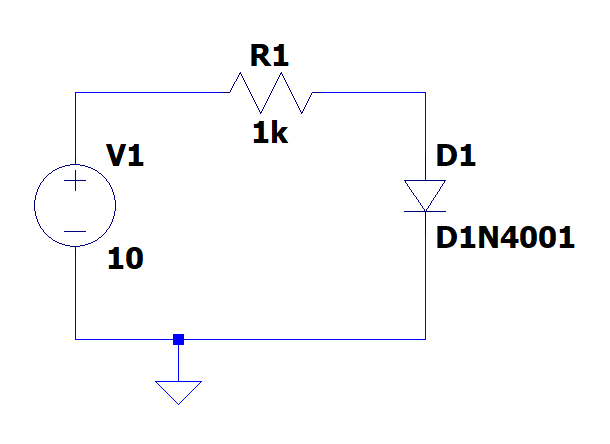
\includegraphics[width=0.7\linewidth]{circuit.png}
  \caption{The circuit in LTSpice}
  \label{fig:circuit1}
\end{figure} 

\section{Summary}
Overall, the best model for diodes is the exponential, but constant
drop is easier to use, so we often use that one.

\end{document}